\documentclass[a4paper,12pt]{report}
%\documentclass[12pt]{uafthesis}


%allows for hyperlink
\usepackage{hyperref}

%\usepackage{url}

%allows for degree symbol, among other things presumably
\usepackage{textcomp}

%draws bounding boxes around the major page elements. For troubleshooting
%\usepackage[showframe]{geometry}
\usepackage[margin=0.2in]{geometry}

%Allows for drawing circuit diagrams
%\usepackage[siunitx]{circuitikz}
\usepackage[american]{circuitikz}

\usepackage{multirow}

\usepackage{amsmath, amssymb, amsfonts} % Thanks, AMS!
\usepackage{fixltx2e} % Allows \(\) in captions, amongst other things.
%\usepackage{ppl} % The Paladino font (tough to find?)
%\usepackage{pxfonts} % Paladino-like fonts
\usepackage{graphicx, float} % Graphics stuff
\usepackage{verbatim} % Mostly for the comment environment.
%\usepackage{chapterbib} % This is an option for those bundling papers.
%\usepackage[square]{natbib}
%\usepackage{tocbibind} % This fixes the "bibliography in ToC" problem.
                        % Use with chapterbib.





\begin{document}


%Each table is included

\begin{figure}[h]
	
\centering
\caption{Simplified diagram of a single phase full-bridge rectifier.}
\label{fig:simple_rectifier}


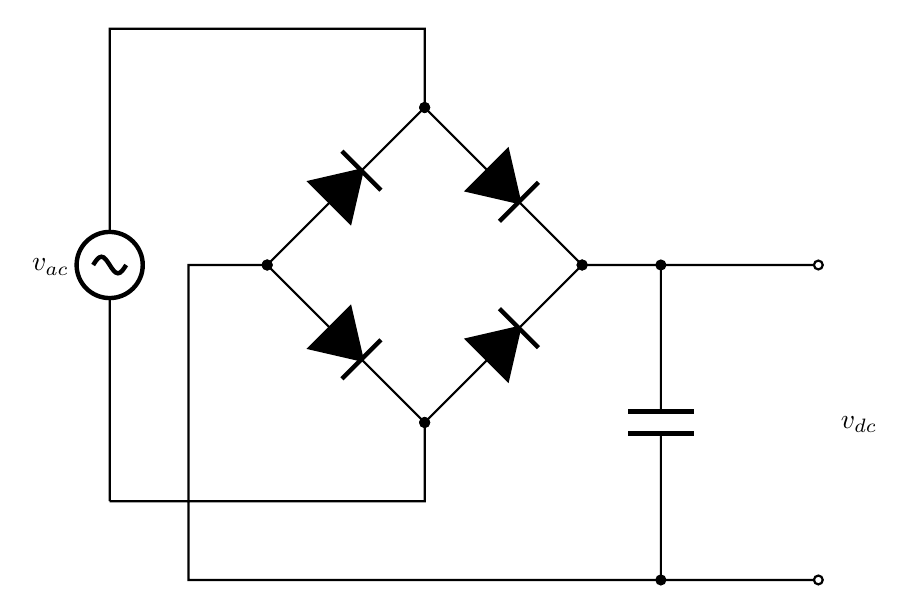
\begin{tikzpicture}
\draw[color=black, thick]
% AC leads
%(0,1) to [short] (4,1) to [short] (4,2){} 
(0,1) -- (4,1) -- (4,2){} 
(0,1) to [sV, l=$v_{ac}$] (0,7) -- (4,7) -- (4,6){}

%Rectifier Diode Bridge
(2,4) to [D*, *-*] (4,6) to [D*, *-*] (6,4){}
(2,4) to [D*, *-*] (4,2) to [D*, *-*] (6,4){}

%DC leads
(2,4) -- (1,4) -- (1,0) to [short, -o] (9,0){}
(6,4) to [short, -o] (9,4){}

%Output 
(7,4) to [C, *-*] (7,0){}
(9,4) to [open, l=$v_{dc}$] (9,0)
;
\end{tikzpicture}

\end{figure}
\begin{figure}[h]
	
\centering

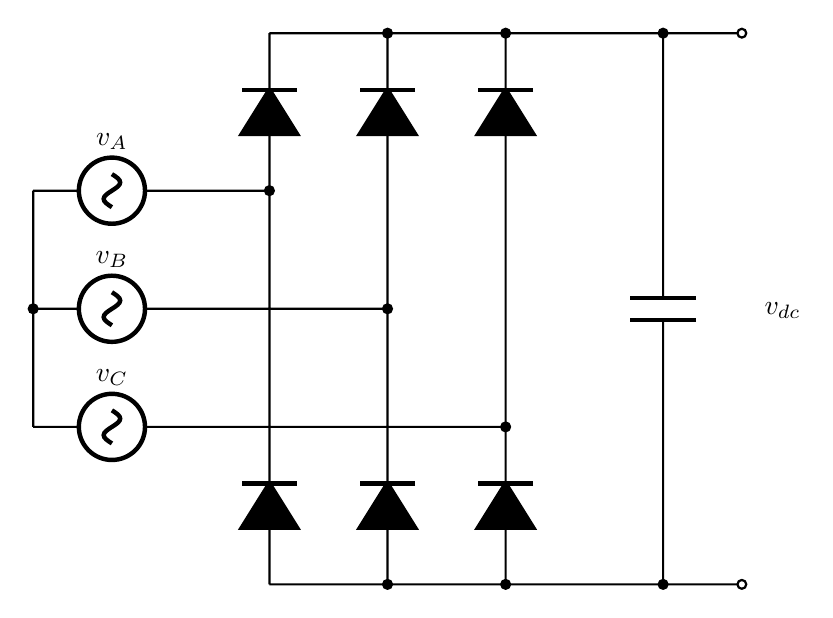
\begin{tikzpicture}
\draw[color=black, thick]
% AC leads
% Wye neutral
(0,2) -- (0,5)

% Three phase voltage sources
(0,5) to [sV, l=$v_A$] (2,5) to [short, -*] (3,5){}
(0,3.5) to [sV, l=$v_B$, *-] (2,3.5) to [short, -*] (4.5,3.5){}
(0,2) to [sV, l=$v_C$] (2,2) to [short, -*] (6,2){}

% A ph diodes
(3,0) to [D*] (3,2) -- (3,5) to [D*] (3,7){}

% B ph diodes
(4.5,0) to [D*, *-] (4.5,2) -- (4.5,5) to [D*, -*] (4.5,7){}

% C ph diodes
(6,0) to [D*, *-] (6,2) -- (6,5) to [D*, -*] (6,7){}


%DC leads
(3,7) to [short, -o] (9,7){}
(3,0) to [short, -o] (9,0){}

%Output 
(8,7) to [C, *-*] (8,0){}
(9,7) to [open, l=$v_{dc}$] (9,0)
;
\end{tikzpicture}

\caption{Simplified diagram of a three phase full-bridge rectifier.}
\label{fig:3ph_rectifier}

\end{figure}
\begin{figure}[h]
	
\centering

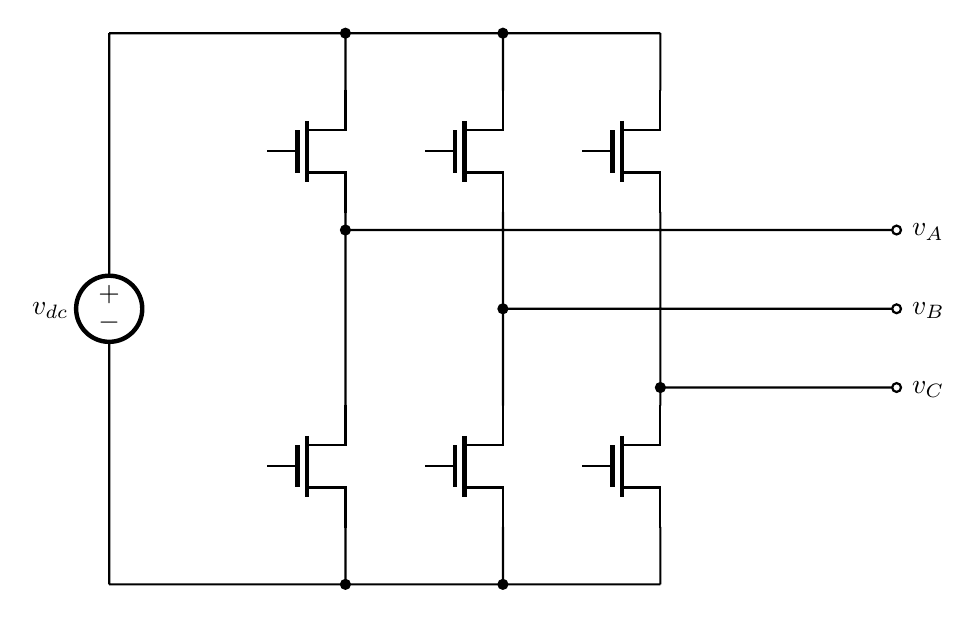
\begin{tikzpicture}
\draw[color=black, thick]
%DC leads
(0,0) -- (7,0){}
(0,7) -- (7,7){}

%Input 
%(1,7) to [C, *-*] (1,0){}
(0,7) to [V, l_=$v_{dc}$] (0,0)

%A switches
(3,5.5) node[nmos] (mos) {}
(mos.gate) node[anchor=east] {}
(mos.drain) to [short, -*] (3,7){}
(mos.source) -- (3,4.5) to [short, *-o] (10,4.5) to [short, l_=$v_{A}$] (10,4.5){}

(3,1.5) node[nmos] (mos) {}
(mos.gate) node[anchor=east] {}
(mos.drain) -- (3,4.5){}
(mos.source) to [short, -*] (3,0){}

%B switches
(5,5.5) node[nmos] (mos) {}
(mos.gate) node[anchor=east] {}
(mos.drain) to [short, -*] (5,7){}
(mos.source) -- (5,3.5) to [short, *-o] (10,3.5) to [short, l_=$v_{B}$] (10,3.5){}

(5,1.5) node[nmos] (mos) {}
(mos.gate) node[anchor=east] {}
(mos.drain) -- (5,3.5){}
(mos.source) to [short, -*] (5,0){}

%C switches
(7,5.5) node[nmos] (mos) {}
(mos.gate) node[anchor=east] {}
(mos.drain) -- (7,7){}
(mos.source) -- (7,2.5) to [short, *-o] (10,2.5) to [short, l_=$v_{C}$] (10,2.5){}

(7,1.5) node[nmos] (mos) {}
(mos.gate) node[anchor=east] {}
(mos.drain) -- (7,2.5){}
(mos.source) -- (7,0){}


;
\end{tikzpicture}

\caption{Simplified diagram of a three phase inverter.}
\label{fig:3ph_inverter}

\end{figure}
\begin{figure}[h]
	
\centering

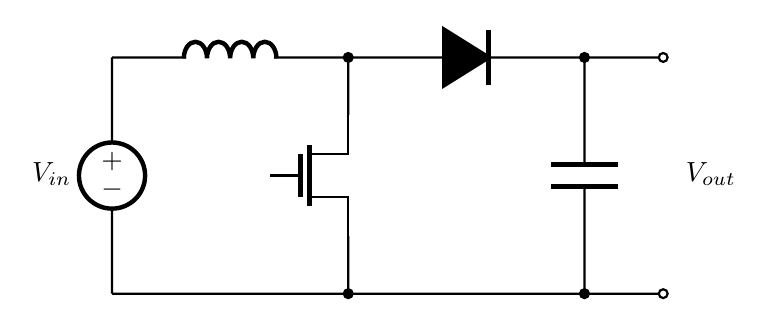
\begin{tikzpicture}[american voltages]
\draw[color=black, thick]
%Input
(0,0) to [V, l=$V_{in}$, invert] (0,3){}

%high 
(0,3) to [L] (3,3) to [D*] (6,3) -- (7,3){}

%switch
(3,1.5) node[nmos] (mos) {}
(mos.gate) node[anchor=east] {}
(mos.drain) to [short, -*] (3,3){}
(mos.source) to [short, -*] (3,0){}

%low
(0,0) -- (7,0){}

%output
(7,3) to [open, l=$V_{out}$, o-o] (7,0){}
(6,3) to [C, *-*] (6,0){}
;
\end{tikzpicture}
\caption{Simplified diagram of a boost converter.}
\label{fig:simple_boost}


\end{figure}
\begin{figure}[h]
	
\centering


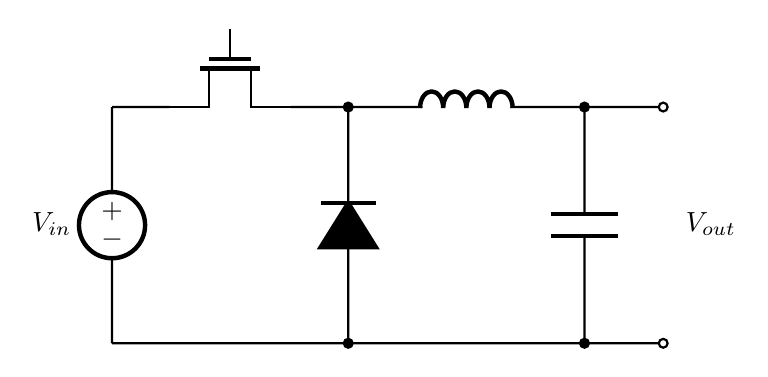
\begin{tikzpicture}[american voltages]
\draw[color=black, thick]
%Input
(0,0) to [V, l=$V_{in}$, invert] (0,3){}

%high 
(3,3) to [L] (6,3) -- (7,3){}

%switch
(0,3) to [Tnmos] (3,3) {}

%Diode
(3,0) to [D*, *-*] (3,3){}

%low
(0,0) -- (7,0){}

%output
(7,3) to [open, l=$V_{out}$, o-o] (7,0){}
(6,3) to [C, *-*] (6,0){}
;
\end{tikzpicture}
\caption{Simplified diagram of a buck converter.}
\label{fig:simple_buck}

\end{figure}
\begin{figure}[h]
	
\centering

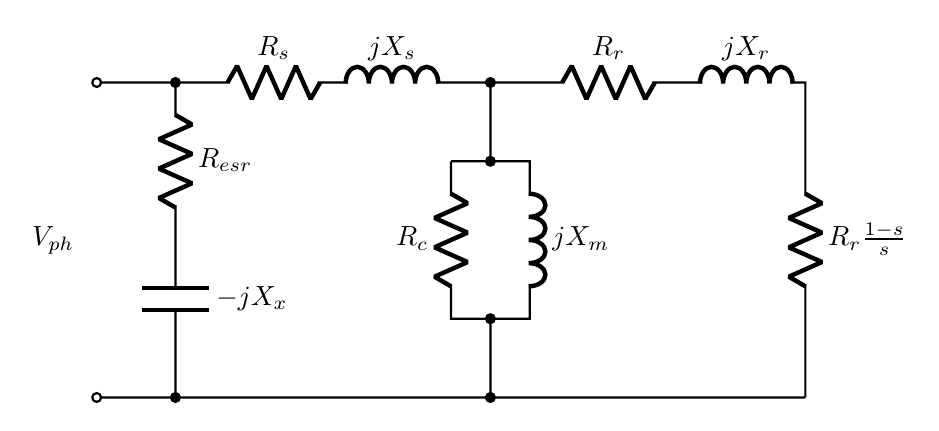
\begin{tikzpicture}[american voltages]
\draw[color=black, thick]
%Input
(0,0) to [open, l=$V_{ph}$, o-o] (0,4){}

%low
(0,0) -- (9,0){}

%stator
(0,4) -- (1.5,4) to [R, l=$R_{s}$] (3,4) to [L, l = $j X_{s}$] (4.5,4){}

%rotor
(4.5,4) -- (5.5,4) to [R, l=$R_{r}$] (7.5,4) to [L, l = $j X_{r}$] (9,4) to [R, l=$R_{r}\frac{1-s}{s}$] (9,0){}

%core
(5,4) to [short, *-*] (5,3){}
(4.5,3) -- (5.5,3) to [L, l = $j X_{m}$] (5.5,1) -- (4.5,1) to [R, l=$R_{c}$] (4.5,3){}
(5,1) to [short, *-*] (5,0){}

%external excitaion capacitor
(1,4) to [R, l=$R_{esr}$, *-] (1,2) to [C, l=$-j X_x$] (1,0.5) to [short, -*] (1,0){}


;
\end{tikzpicture}

\caption{Single phase diagram of a three phase squirrel cage induction machine. $V_{ph}$ and $s$ are the phase voltage and slip of the generator. }
\label{fig:SCIG__circuit_diagram}

\end{figure}
\begin{figure}[h]
	\centering
	\caption{A simplified diagram of power and data flows of the model. Blue lines represent electrical power connections and flows similar to a one-line diagram. Green boxes represent data flow from one part of the model to another.}
	\label{fig:abridged_flow_diagram_label}
	
	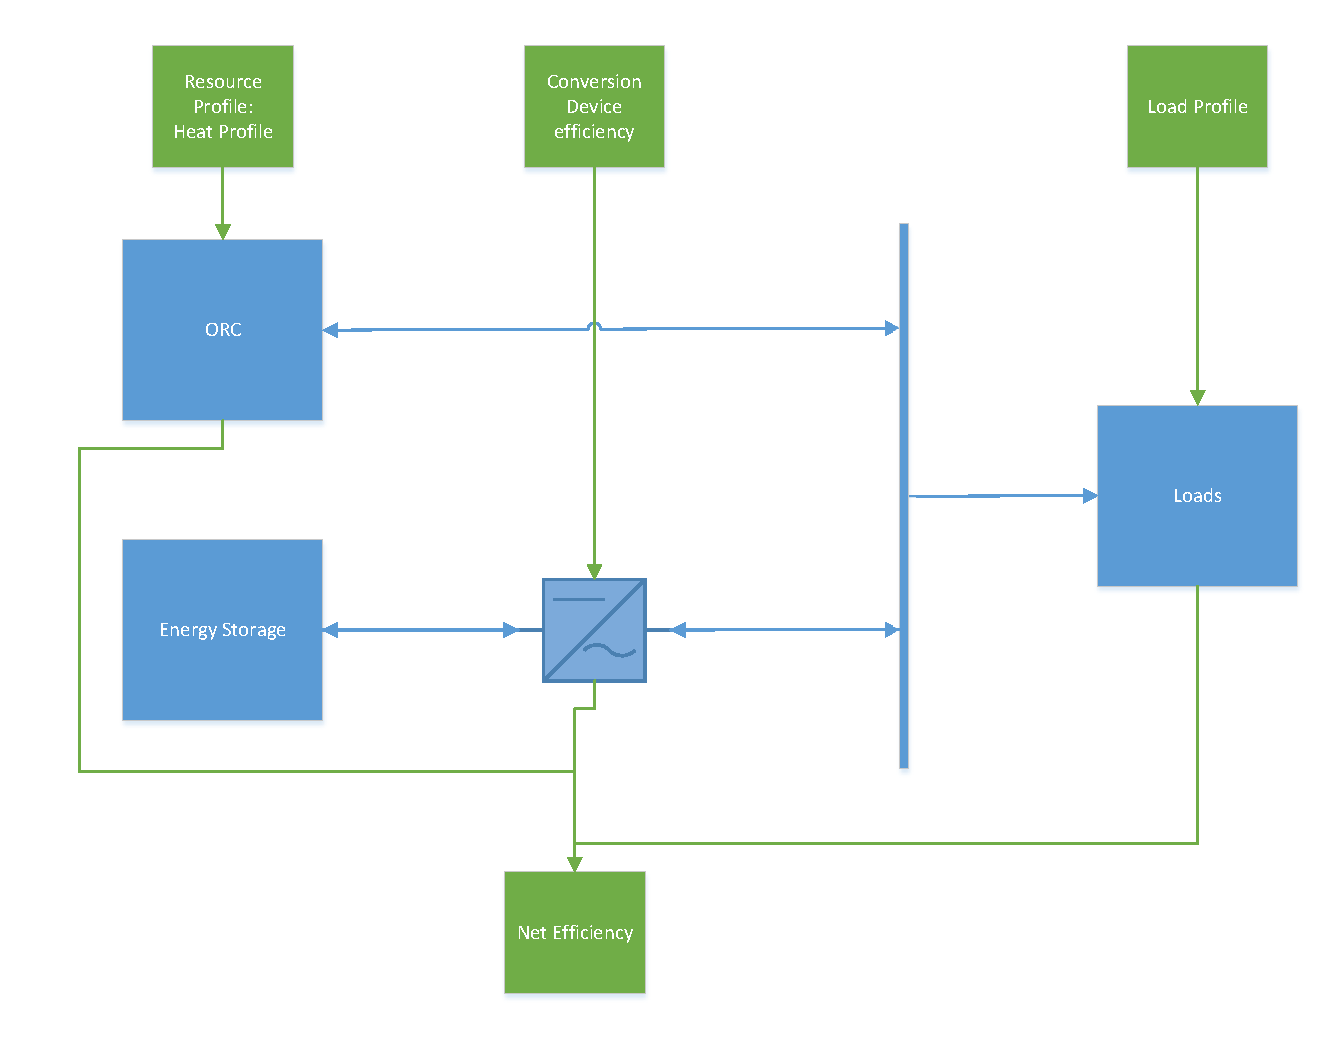
\includegraphics[width=\textwidth]{figures/Abridged Pilgrim Model Flow diagram - AC bus.pdf} 
	%\includegraphics[width=\textwidth]{figures/SimpleFlowDiagram.pdf}

\end{figure}
\begin{figure}[h]
	\centering

	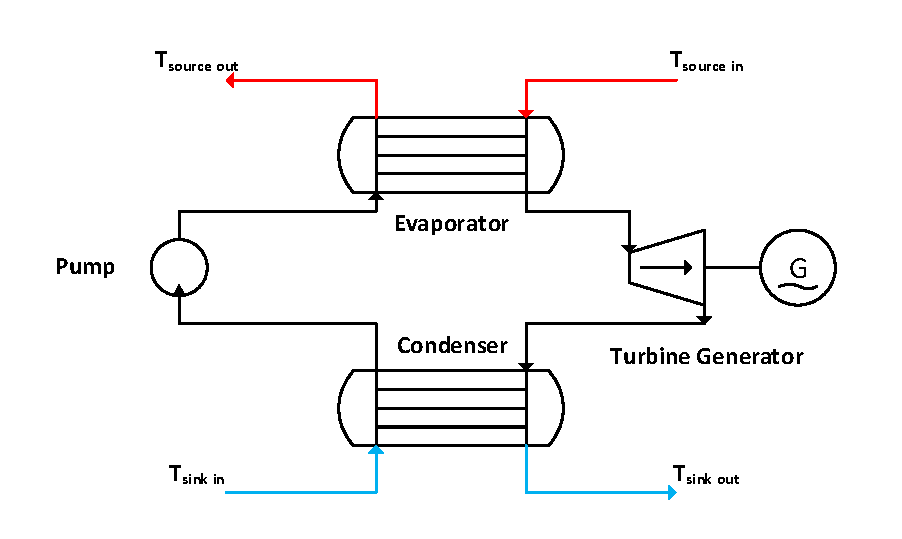
\includegraphics[width=\textwidth]{figures/RankineCycleDiagram.pdf}

	\caption{Diagram of a Rankine cycle system.}
	\label{fig:rankine_cycle_diagram}
	
\end{figure}
%\begin{figure}[h]
	\centering

	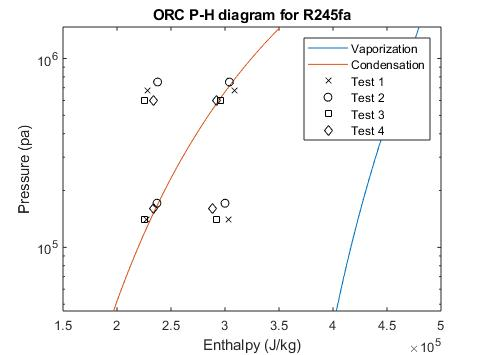
\includegraphics[width=\textwidth]{figures/VerificationPH01}
	%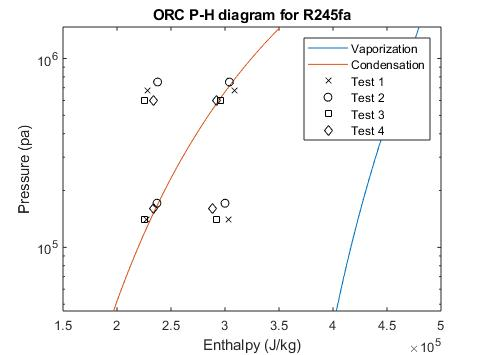
\includegraphics{figures/VerificationPH01}

	\caption{Pressure-Enthalpy plot of R245-fa for ORC verification. 
	For tests 1 \& 2 $T_{source}$ is about \SI{364}{\kelvin} (\SI{195}{\degreeFahrenheit})
	while for 3 \& 4 $T_{source}$ is \SI{353}{\kelvin} (\SI{175}{\degreeFahrenheit}). 
	In all cases $T_{sink}$ is about \SI{283}{\kelvin} (\SI{50}{\degreeFahrenheit}). 
	The hot water flow rate for tests 1 \& 3 are \SI{18.9}{\liter\per\second} (\SI{300}{\gpm})
	and	\SI{7.6}{\liter\per\second} (\SI{120}{\gpm}) for test 2 \& 4. 
	The cold water flow rate for tests 1 \& 3 are \SI{12.6}{\liter\per\second} (\SI{200}{\gpm})
	and \SI{7.6}{\liter\per\second} (\SI{120}{\gpm}) for test 2 \& 4.}
	\label{fig:verifcation_ph01}
\end{figure}
%\begin{figure}%[h]
	\centering
	\caption{Pressure-Enthalpy plot of R245-fa for ORC verification with an over sized evaporator area. Input tempetures and flow rates remain the same. 
	For tests 1 \& 2 $T_{source}$ is about \SI{364}{\kelvin} (\SI{195}{\degreeFahrenheit})
	while for 3 \& 4 $T_{source}$ is \SI{353}{\kelvin} (\SI{175}{\degreeFahrenheit}). 
	In all cases $T_{sink}$ is about \SI{283}{\kelvin} (\SI{50}{\degreeFahrenheit}). 
	The hot water flow rate for tests 1 \& 3 are \SI{18.9}{\liter\per\second} (\SI{300}{\gpm})
	and	\SI{7.6}{\liter\per\second} (\SI{120}{\gpm}) for test 2 \& 4. 
	The cold water flow rate for tests 1 \& 3 are \SI{12.6}{\liter\per\second} (\SI{200}{\gpm})
	and \SI{7.6}{\liter\per\second} (\SI{120}{\gpm}) for test 2 \& 4.}
	\label{fig:verifcation_ph02}
	
	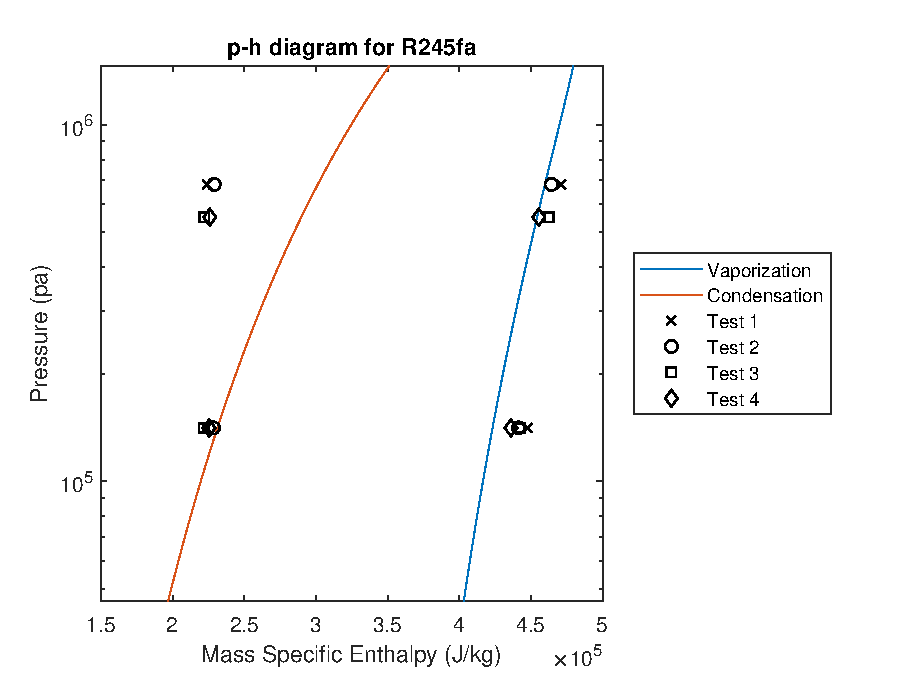
\includegraphics[width=\textwidth]{figures/VerificationPH02}
	%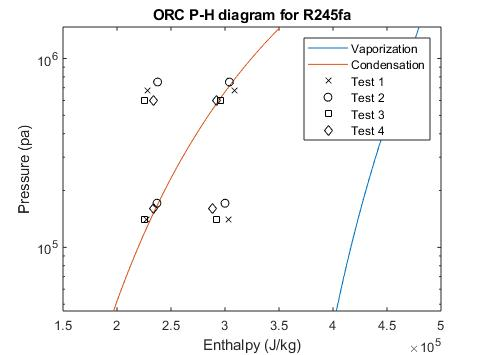
\includegraphics{figures/VerificationPH01}
\end{figure}

\end{document}
